
\title{Security Analysis of Github}
\author{
        Sean Smith, Kyle Holzinger, Amalia Safer\\
}
\date{\today}

\documentclass[12pt]{article}
\usepackage{graphicx}
\usepackage{natbib}
\usepackage{booktabs}
\usepackage{subfigure}
\usepackage{amsmath}
\usepackage{listings}
\usepackage{subfigure}


\usepackage{algpseudocode}
\usepackage{alltt}
\usepackage{textcomp}
\usepackage{url}
\usepackage{amssymb, amsthm, bm}
%\usepackage{semantic}
\usepackage{eso-pic}

\renewcommand{\tt}[1]{\texttt{#1}}
\newcommand{\tts}[1]{\tiny{\texttt{#1}}}
\newenvironment{myprogramtext}
{\begin{list}{}{\setlength{\leftmargin}{1em}}\item\small\bfseries}
{\end{list}}

\renewenvironment{figure}
               {\def\@captype {figure}}
               {}

\renewenvironment{table}
               {\def\@captype {table}}
               {}


\begin{document}
\maketitle

\section{Introduction}
INSERT INTRODUCTION HERE

\section{Cookies}\label{cookies}
	A session cookie called {\tt user\_session} is stored which contains a seemingly random nonce. When a get request is made to {\tt https://github.com}, the cookie is sent and the database is queried to see if the cookie is valid. If the cookie is valid it will return user data as if the user is logged in. There are two more cookies of importance {\tt logged\_in} which is a yes/no value and {\tt dotcom\_user} which is the user's username. To impersonate a user, only the {\tt user\_session} is needed, the {\tt logged\_in} cookie will always be yes and the {\tt dotcom\_user} will be filled by the server if the {\tt user\_session} cookie is valid. When the user logs out, the cookie is invalided by the server in a post request to {\tt https://github.com/logout} that contains the content type and an authenticity token. The authenticity token is a random nonce that github uses to prevent against CSRF. If an attacker is using the user's cookie and the user logs out, the attacker's cookie will be invalidated.

When the user logs in, a post request is sent to {\tt https://github.com/session} with the username, password and authenticity token.

One attack is to guess a random cookie and query to see if it's valid. There are approximately 8 million active github users at a time so roughly 8 million valid cookies. Since you don't need the {\tt logged\_in} cookie to be set correctly, you can construct a random cookie and check if it's valid. The length of the cookie is 80 characters and each character is from the universe (a-z, A-Z, 0-9, -, \_) which has a size of 64. Say the set of correct cookies $S$  has size $|S| = 8,000,000$, the universe $U$ has a size of $|U| = 64^{80}$. The probability of guessing a correct cookie $c$ is so low that it's not a reasonable attack.

$$Pr[c \in S] = \frac{|S|}{|U|} \approx 10^{-138}$$


%Section USER TRACKING
\section{User Tracking}\label{tracking}
Github does not serve ads as it's business model revolves around selling premium subscriptions. However it does track users for analytics purposes via Google analytics. It does this in two ways:

\begin{enumerate}
%1
\item Google analytics sticks cookies on the user's browser. First it sticks a {\tt \_ga} cookie that expires in two years to distinguish between individual users, then it sticks a {\tt \_utma} cookie that expires in 30 years that is updated every time a request is sent to google analytics. 

%2
\item In the rare event that the user removes these cookies, google analytics tries to fingerprint the user. It collects the browser, operating system, extensions installed, model of the computer and a couple other distinguishing factors. This is collected from the {\tt user\_agent} header which contains information such as {\tt Mozilla/5.0 (Macintosh; Intel Mac OS X 10\_10\_2) AppleWebKit/537.36 (KHTML, like Gecko) Chrome/42.0.2311.90 Safari/537.36}. Users who do not allow cookies are even easier to identify than other users as the server identifies that they don't allow cookies and then it's a smaller pool of people that they may be. The remaining identifying information is enough to identify the user. From my browser setup 22 bits of unique identifying information is available. Enough to make me distinct in a pool of $5,000,000$ people.

%\begin{figure}
\begin{table}
\begin{tabular}{| l | p{7cm} | p{7cm} |}
\hline
\textbf{Browser Characteristic} & \textbf{Bits of identifying information} & \textbf{One in x browsers have this} \\ \hline
User Agent                      & 12.92                                    & 7752.4                               \\ \hline
HTTP\_ACCEPT Headers            & 6.72                                     & 105.71                               \\ \hline
Browser Plugin Details          & 11.11                                    & 2205.31                              \\ \hline
Time Zone                       & 4.06                                     & 16.67                                \\ \hline
Screen Size and Color Depth     & 4.18                                     & 18.16                                \\ \hline
System Fonts                    & 17.21                                    & 151725.49                            \\ \hline
Are Cookies Enabled?            & 0.43                                     & 1.35                                 \\ \hline
supercookie test                & 0.86                                     & 1.81                                 \\ \hline
\end{tabular}
\end{table}
%\caption{\newline}
%\label{fig:mig_over}
%\end{figure}


\end{enumerate}

%Section CSP
\section{CSP}
Content security policy or CSP is a way of whitelisting domains that github.com is allowing to load into into the page. This whitelist contains the.\\

\begin{figure}
\begin{table}
\begin{tabular}{| l | l | l | l | l | }
\hline

Subdomain & Visitors & Percent of Daily Traffic \\ \hline
github.com & 12,910,000 & 85.34\% \\ \hline
gist.github.com & 1,237,000 & 8.18\%  \\ \hline
help.github.com & 330,600 & 2.19\%  \\ \hline
codeload.github.com & 206,500 & 1.37\%  \\ \hline
twitter.github.com & 106,600 & 0.7\%  \\ \hline
status.github.com & 89,100 & 0.59\%  \\ \hline
windows.github.com & 87,700 & 0.58\%  \\ \hline
divshot.github.com & 59,400 & 0.39\%  \\ \hline
guides.github.com & 56,700 & 0.37\%  \\ \hline
fortawesome.github.com & 44,500 & 0.29\%  \\ \hline
\end{tabular}
\end{table}
\caption{\newline}
\label{fig:mig_over}
\end{figure}


\section{SSL Everywhere}

All connections to github.com are done via https. This is enforced via HTTP strict transport security (HSTS). Github sets the {\tt Strict-Transport-Security} header to {\tt max-age=31536000; includeSubdomains; preload}. This ensures that for the next year, the browser will only accept connections from github.com over SSL. To further this Github is now included in the chrome STS file. This is a file that ships with Chrome and ensures that whenever Chrome goes to \url{github.com} it will only accept connections over SSL. Since Chrome is open source we dug up the STS (strict transport security) file and found the entry that corresponds to Chrome.

{\tt \{ "name": "github.com", "include\_subdomains": true, "mode": "force-https" \}}


\section{Git Commit Attack}
Github relies on the security of Git which has much more security flaws than SSL. We demonstrate an attack the takes advantage of git (github) passwords stored in the clear.

\begin{figure}
\centering
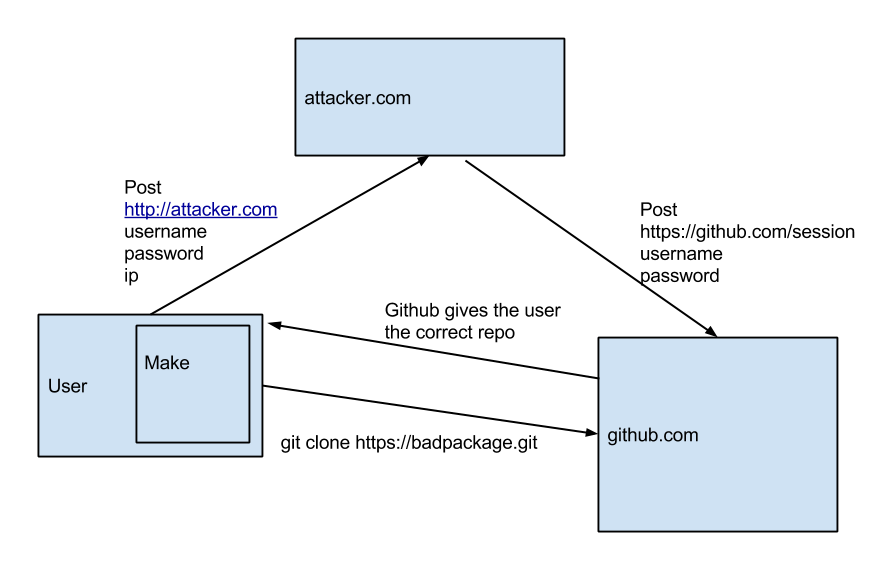
\includegraphics[scale=.5]{attack.png}
\caption{Diagram of our attack\newline}
\label{fig:mig_over}
\end{figure}

\begin{enumerate}
\item First the user clones the repository using the command\\ {\tt git clone https://kholzinger:<password>@github.com/kylelh/linkeffects}
\item Then the user runs the Makefile, a standard procedure on any operating system.\\
{\tt make}

\item The {\tt Makefile} parses the git username and password which are stored in {\tt .git/config} file. The git username and password are also the {\tt github.com} username and password.
\item We send the username, password, and ip address to the command and control server. We can then log into the users account.


\end{enumerate}

\section{XSS}

Github has two major protections against cross-site-scripting (XSS) attacks. 




\section{References}\label{references}
\begin{enumerate}
\item We used this this online tool to fingerprint the browser much in the same way that Google Analytics does.\\ \url{https://panopticlick.eff.org/index.php?action=log&js=yes}
\end{enumerate}
\end{document}
This is never printed